\subsection{Case study}\label{subsec:case-study}
This section describes the practical experiment used to evaluate representations.
The goal was to validate the previous evaluation in a more realistic development scenario.
Additionally, this was an opportunity to \todo{lepszy zwrot} gain an impression of developer experience while using the notations.

\subsubsection{Scenario and context}
The goal of this experiment was to evaluate the expressiveness of representations in a practical context.
This was achieved by recreating a few screens of a fictional application.
The application designed for this experiment was modeled after Trello\furl{trello.com} \textendash\ a well-known Web application for creating Kanban-style lists.
The choice was motivated by the application's popularity and relative complexity.

Capabilities of the original are very broad and include detailed management of workspaces, users, boards, as well as editing and managing content-rich cards.
It would not be reasonable to implement all these functionalities \textendash\ to keep the experiment manageable, it was necessary to limit its scope.
The selected area to implement concerns simple management of cards across two views and a single dialog window:
\begin{itemize}
    \item the first view allows for viewing all boards the user has access to and navigating to a board
    \item the second view allows for viewing a particular board and its data \textendash\ name, columns and cards
    \item the dialog window allows for adding or editing a single card
\end{itemize}
This setup covers all four CRUD operations, making the experiment representative of real-life applications.
Management of boards and columns within a board was omitted to keep the example as small as possible.

Additionally, the representations should be able to represent two major components:
\begin{itemize}
    \item a card \textendash\ contains information about a title of a task, its description, assigned person and due date; it is also assigned to a column
    \item a column \textendash\ a board consists of multiple columns, each possibly containing multiple cards; additionally, to give it meaning, it also has a title
\end{itemize}

To further simplify the experiment, the interface was only implemented in a mobile version \textendash\ it is considered a good practice to design applications and website using the \enquote{mobile first} principle\furl{https://developer.mozilla.org/en-US/docs/Web/Progressive_web_apps/Responsive/Mobile_first}.% \textendash\ focusing on designing for narrow devices in the first place and extending the design from there.

The subsequent paragraphs provide a descriptions of functionalities that the representations were expected to implement.
However, in this case study, the requirements were not prescriptive \textendash\ they only listed \enquote{features} to implement, without specifying how should they be implemented.
This is meant to produce a more practical evaluation.

\todo[inline]{scoring system}

\paragraph{The boards view}
The boards view consists of\textellipsis
\todo[inline]{todo}

\paragraph{The board view}
The board view, presented in figure~\ref{fig:3-4-board-view} consists of a title and multiple columns.
Only the part with the green background is visible to the user;
the rest of the columns need to be scrolled to the view to be visible.

\begin{figure}
    \centering
    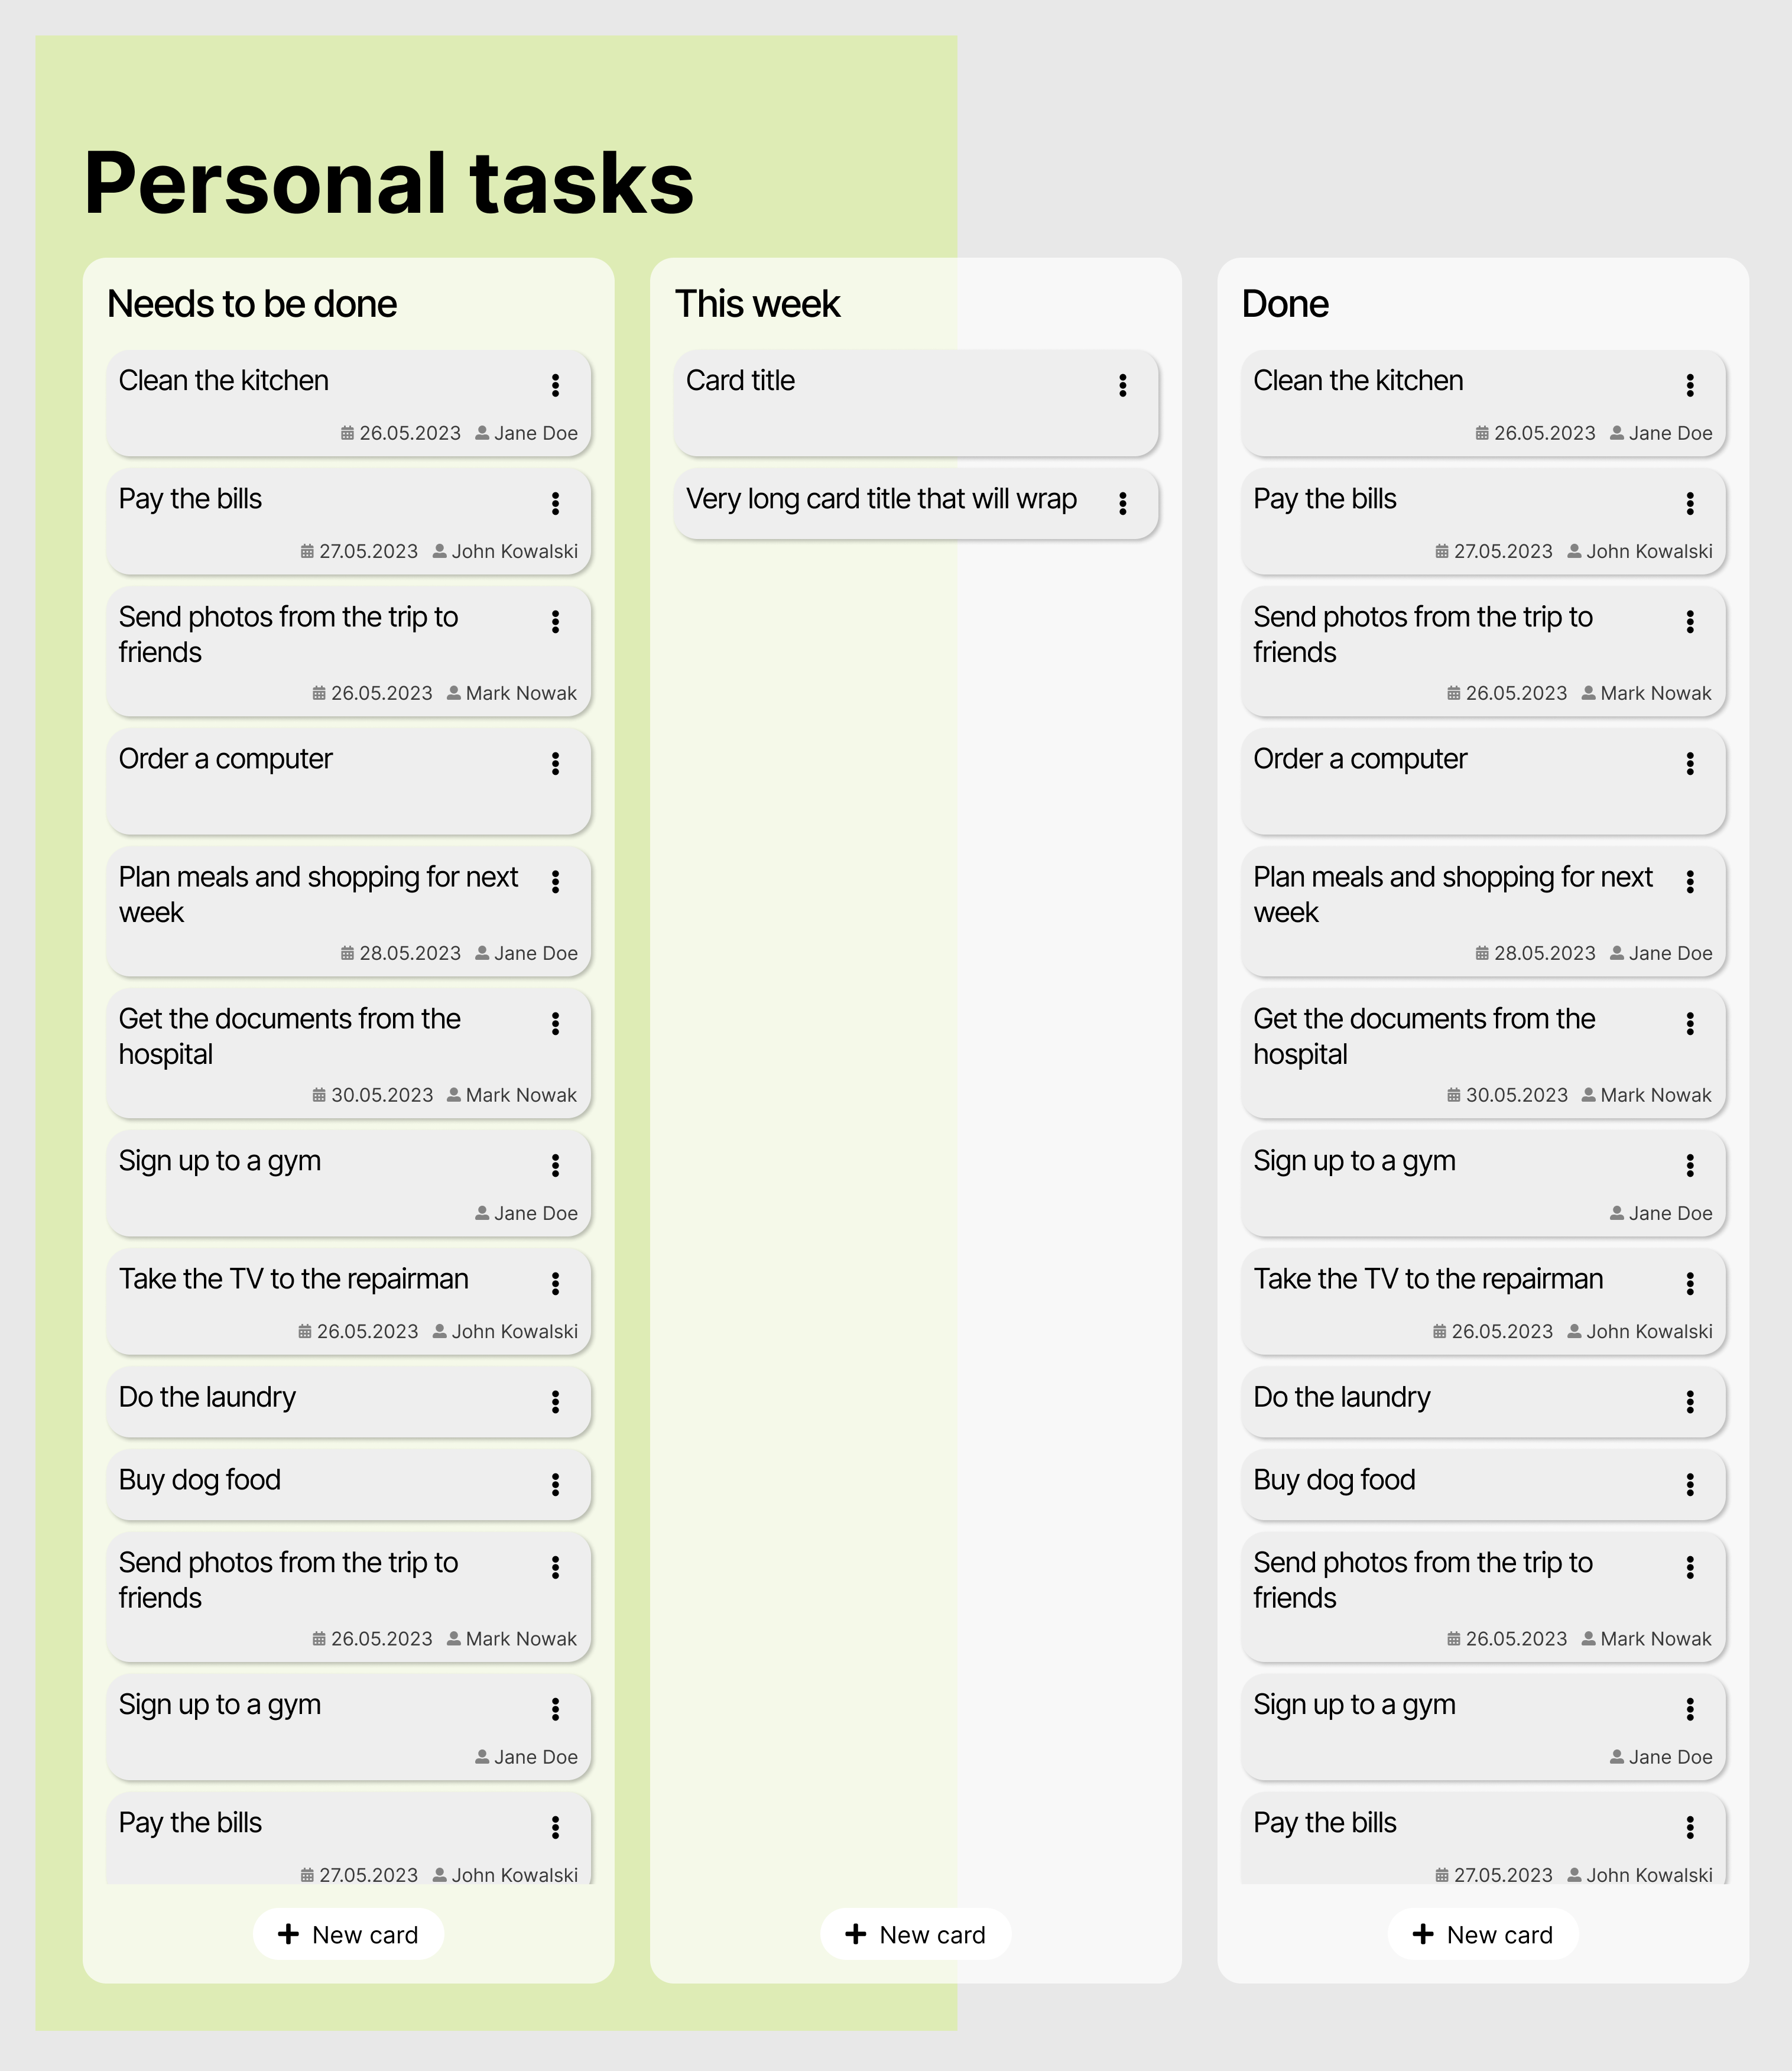
\includegraphics[height=0.4\textheight]{./3-research-methodology/board-view}
    \caption{An example design of a board view.}
    \label{fig:3-4-board-view}
\end{figure}

\paragraph{The column component}
The column component, presented in figure~\ref{fig:3-4-column-component} consists of a title and cards.

\begin{figure}
    \centering
    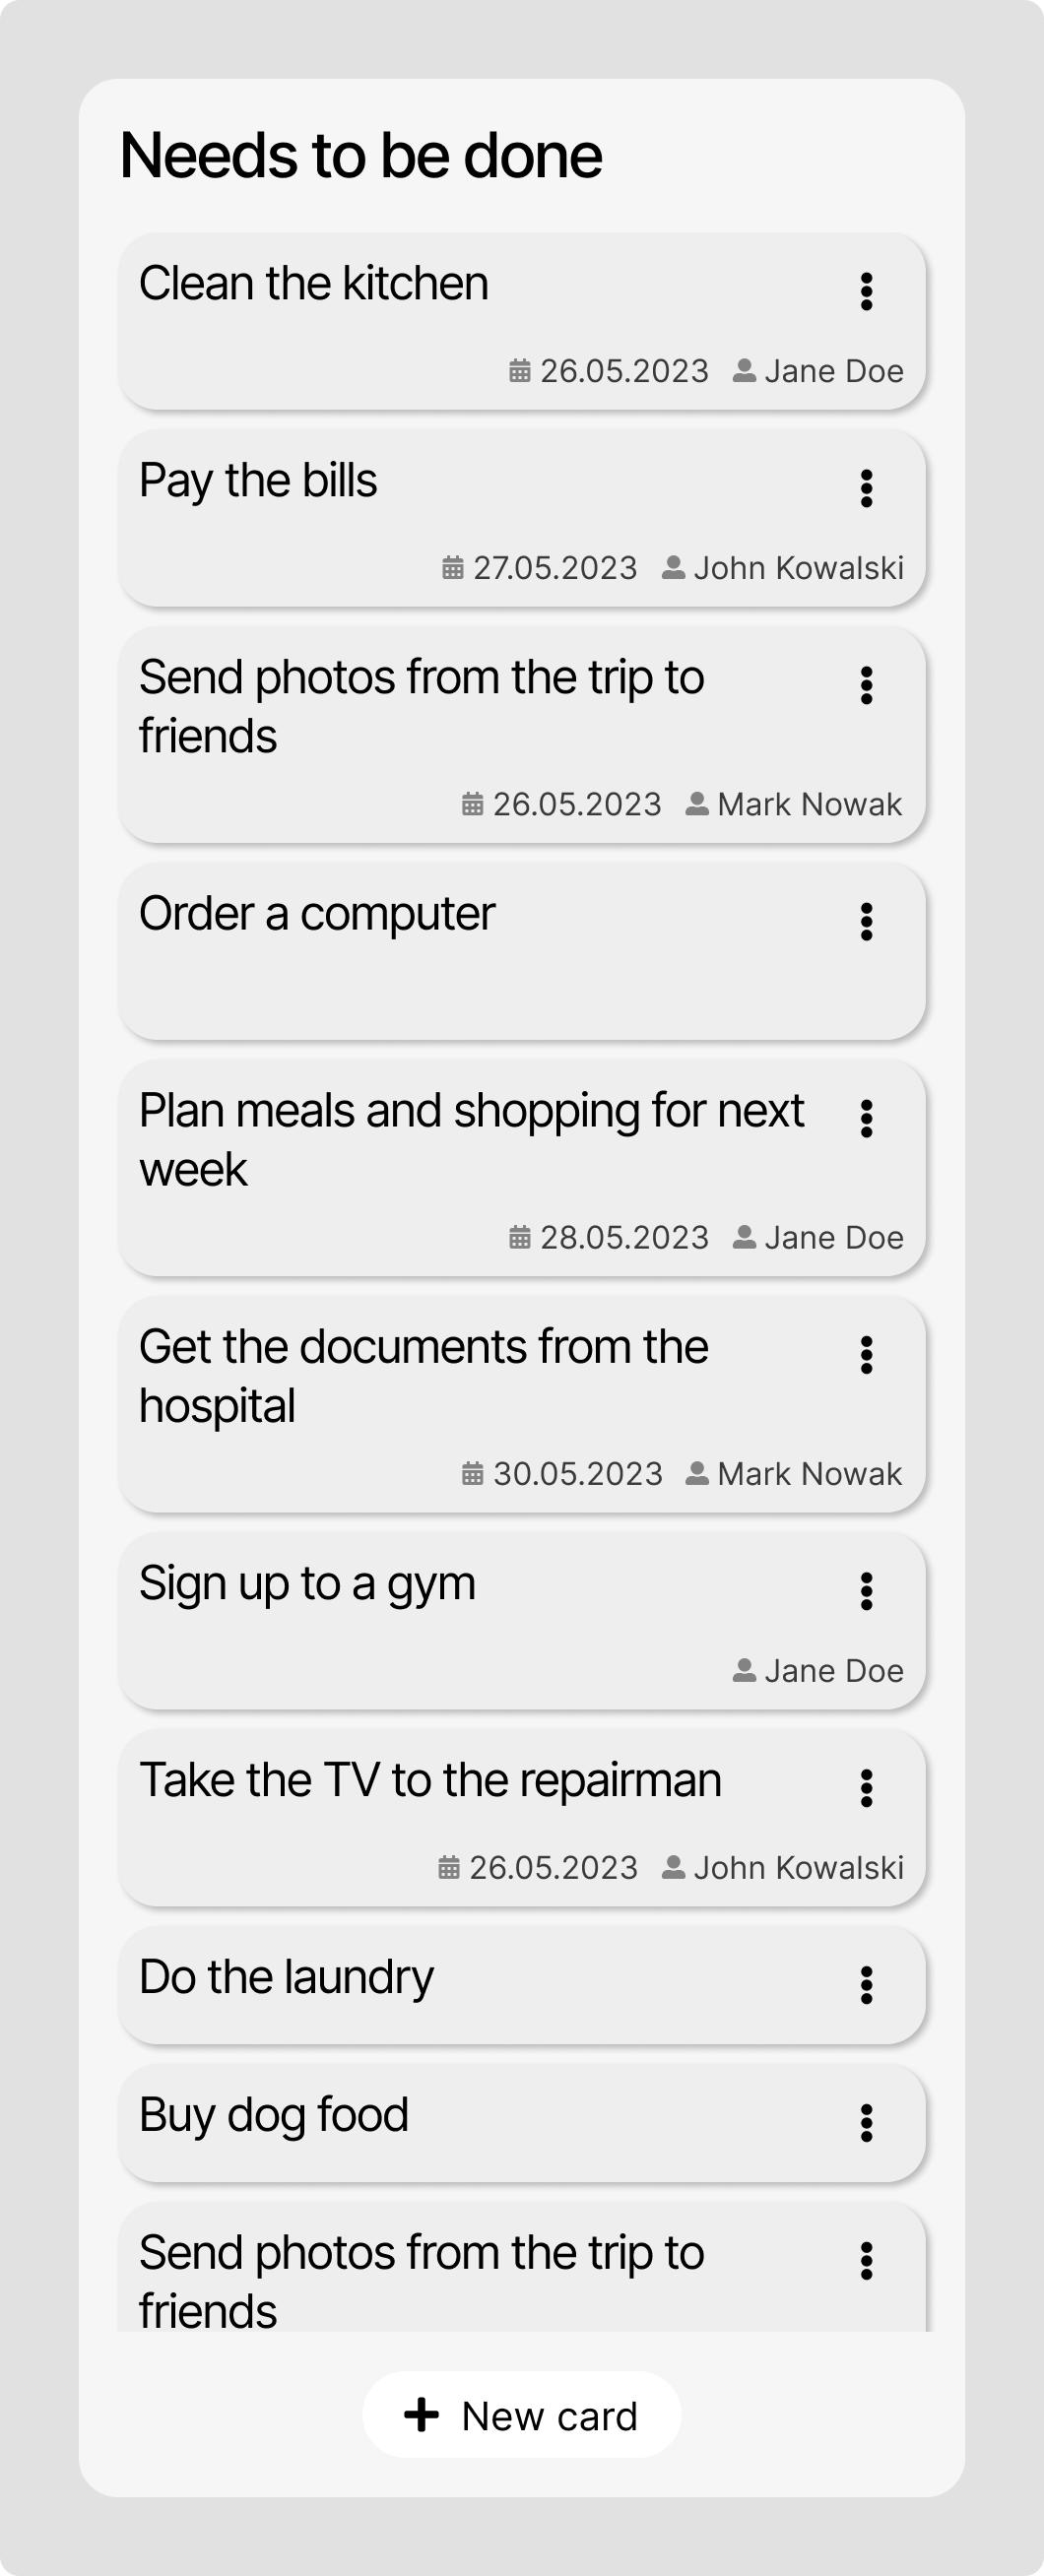
\includegraphics[height=0.5\textheight]{./3-research-methodology/column-component}
    \caption{An example design of a column component.}
    \label{fig:3-4-column-component}
\end{figure}

\paragraph{The card component}
Figure~\ref{fig:3-4-card-component} depicts a card component, consisting of a title and various indicators (short texts with an icon) \textendash\ that unobtrusively signal information about a list item.
\begin{figure}
    \centering
    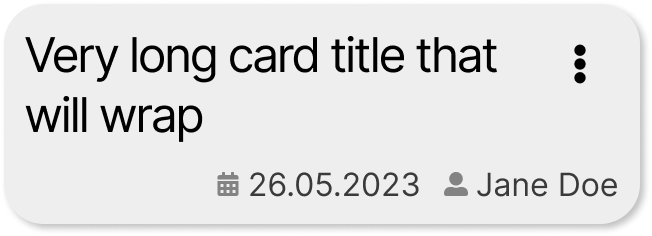
\includegraphics[width=\textwidth]{./3-research-methodology/card-component}
    \caption{An example design of a card component.}
    \label{fig:3-4-card-component}
\end{figure}

The table~\ref{tab:3-4-card-component-requirements} presents the requirements for a card component implemented by the selected representations.

\begin{longtblr}[
    caption = {Requirements for the card component in the case study.},
    label = {tab:3-4-card-component-requirements},
]{
    colspec = {cX[4,c]X[1,c]},
    rowhead = 1,
    rows = {m},
}
    \hline[1pt]
    \textbf{No.} & \textbf{Requirement}                                             & \textbf{Relevant criteria} \\*
    \hline[1pt]
    E1           & the card indicators are displayed using icons                    & \textbf{A6}                \\*
    E2           & the component emits a \texttt{click} event when clicked          & B4.2, B12.4                \\*
    E3           & the component accepts card title and indicators as inputs        & B12.2                      \\*
    E4           & the card has rounded borders                                     & D6.7                       \\*
    E5           & the title takes the whole width of a card and wraps as necessary & \textbf{D3}                \\*
    E6           & the title is displayed in a 12pt font                            & D7.5                       \\*
    E7           & etc\textellipsis                                                 & \textellipsis              \\*
    \hline[1pt]
\end{longtblr}

\paragraph{The card editing dialog}
The dialog is presented in the figure~\ref{fig:3-4-card-editing-dialog}.

\begin{figure}
    \centering
    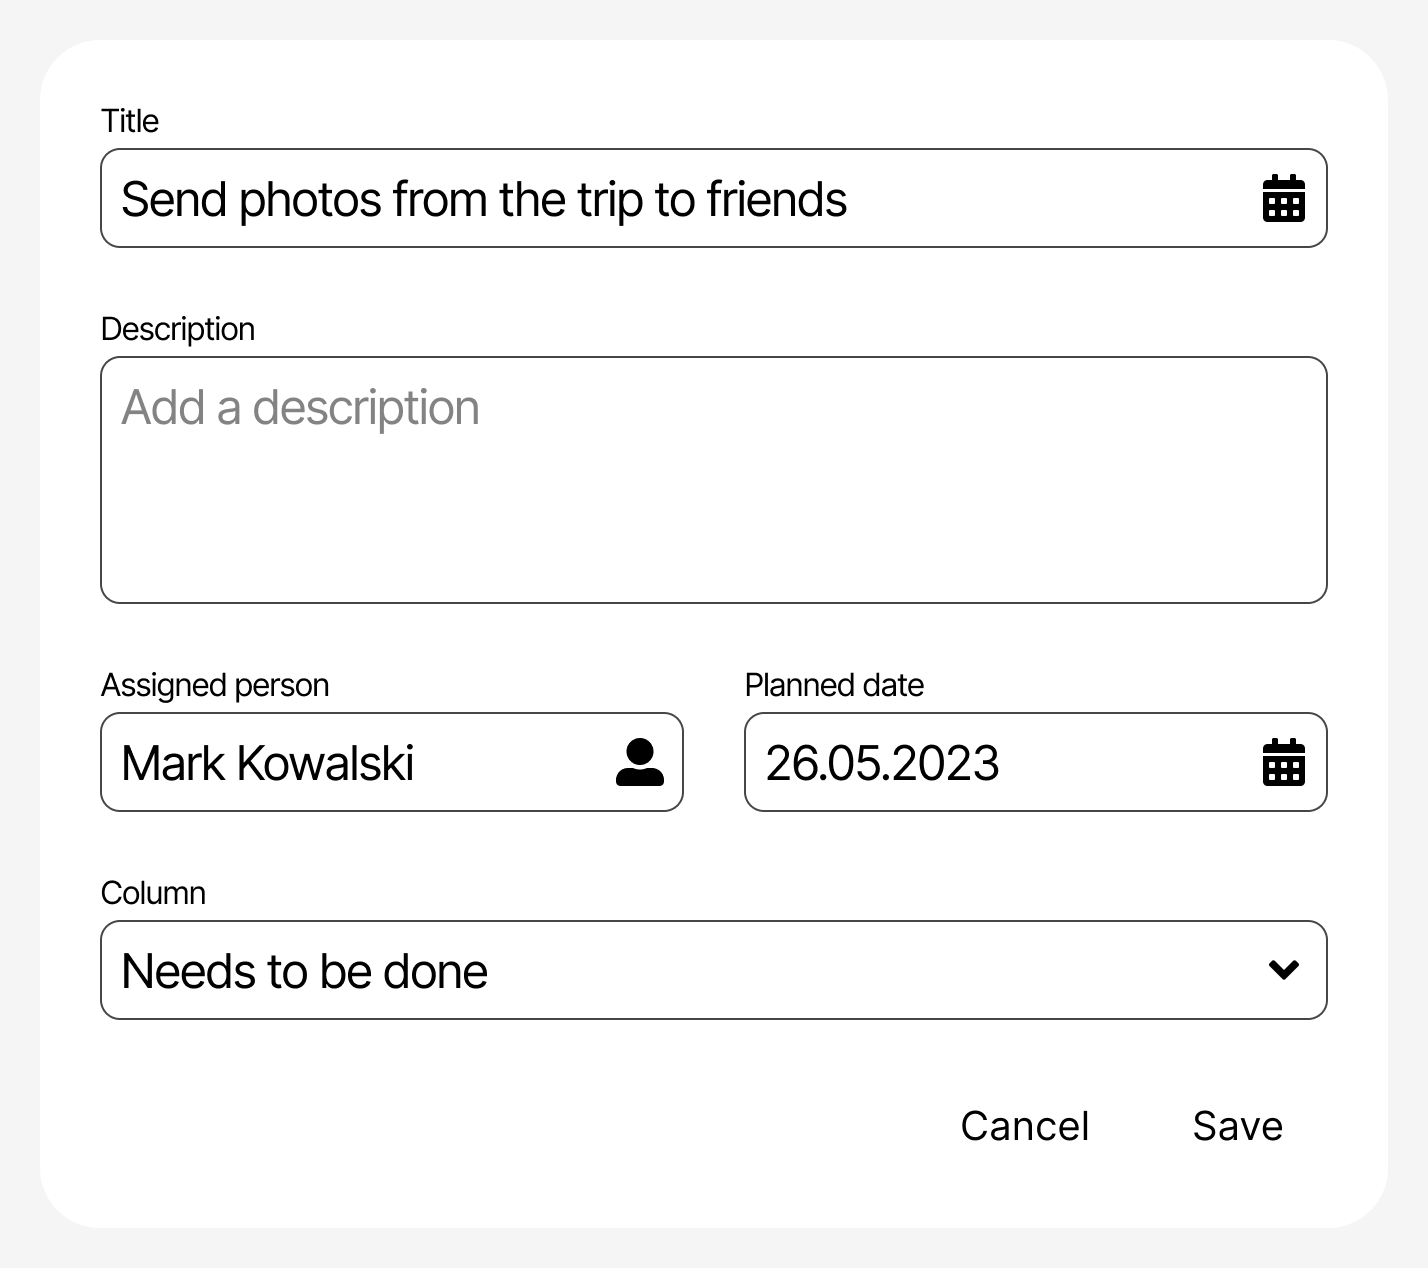
\includegraphics[height=0.4\textheight]{./3-research-methodology/card-editing-dialog}
    \caption{An example design of a card editing dialog.}
    \label{fig:3-4-card-editing-dialog}
\end{figure}
